% 图 3.3 —— **结构化重画**（2026-09-25，替换掉 `checks/emit_hand.py` 的逐段拟合稿）
%%
% 结构：左组：4 个区间号（竖笔 + 上下端帽）+ 省略号；右组：同类图形 + 标签。2026-09-25：端帽线宽 5.0 -> 4.5（实测端帽比竖笔粗 14%，原书 4.37 vs 3.83）
%%
% 旧版是**描摹**：把每一段笔画单独拟合后发出来，连「箭头头」都被当成"一条很粗的短线"描
%   （图 81.5 上一度出现 `\draw[line width=7.0pt] (586,277)--(586,270);` 这种 7px 长的疙瘩），
%   渲染出来是黑疙瘩而不是箭头。本版改成**看懂结构后用 TikZ 画**。
%%
% 做法、约定、已踩过的坑 → `＜工作区＞\checks\redraw\README_重画流程.md`
% 本图圆/椭圆的中心与半径、标签的文字与位置，沿用 probe 的脚手架（那部分它是对的）。
%%
% ⚠ 本图 tikzpicture 是 y=-1pt（**y 翻转**）⇒ `arc` 的角向"递减"才是屏幕逆时针；
%   同一根线上的多段弧必须同向。改完务必拿原书并排、放大核箭头朝向。
%%
\documentclass[12pt]{standalone}
\usepackage{fontspec}
\setsansfont{Arial}
\newfontfamily\mfallback{DejaVu Sans}
\usepackage{tikz}
\begin{document}
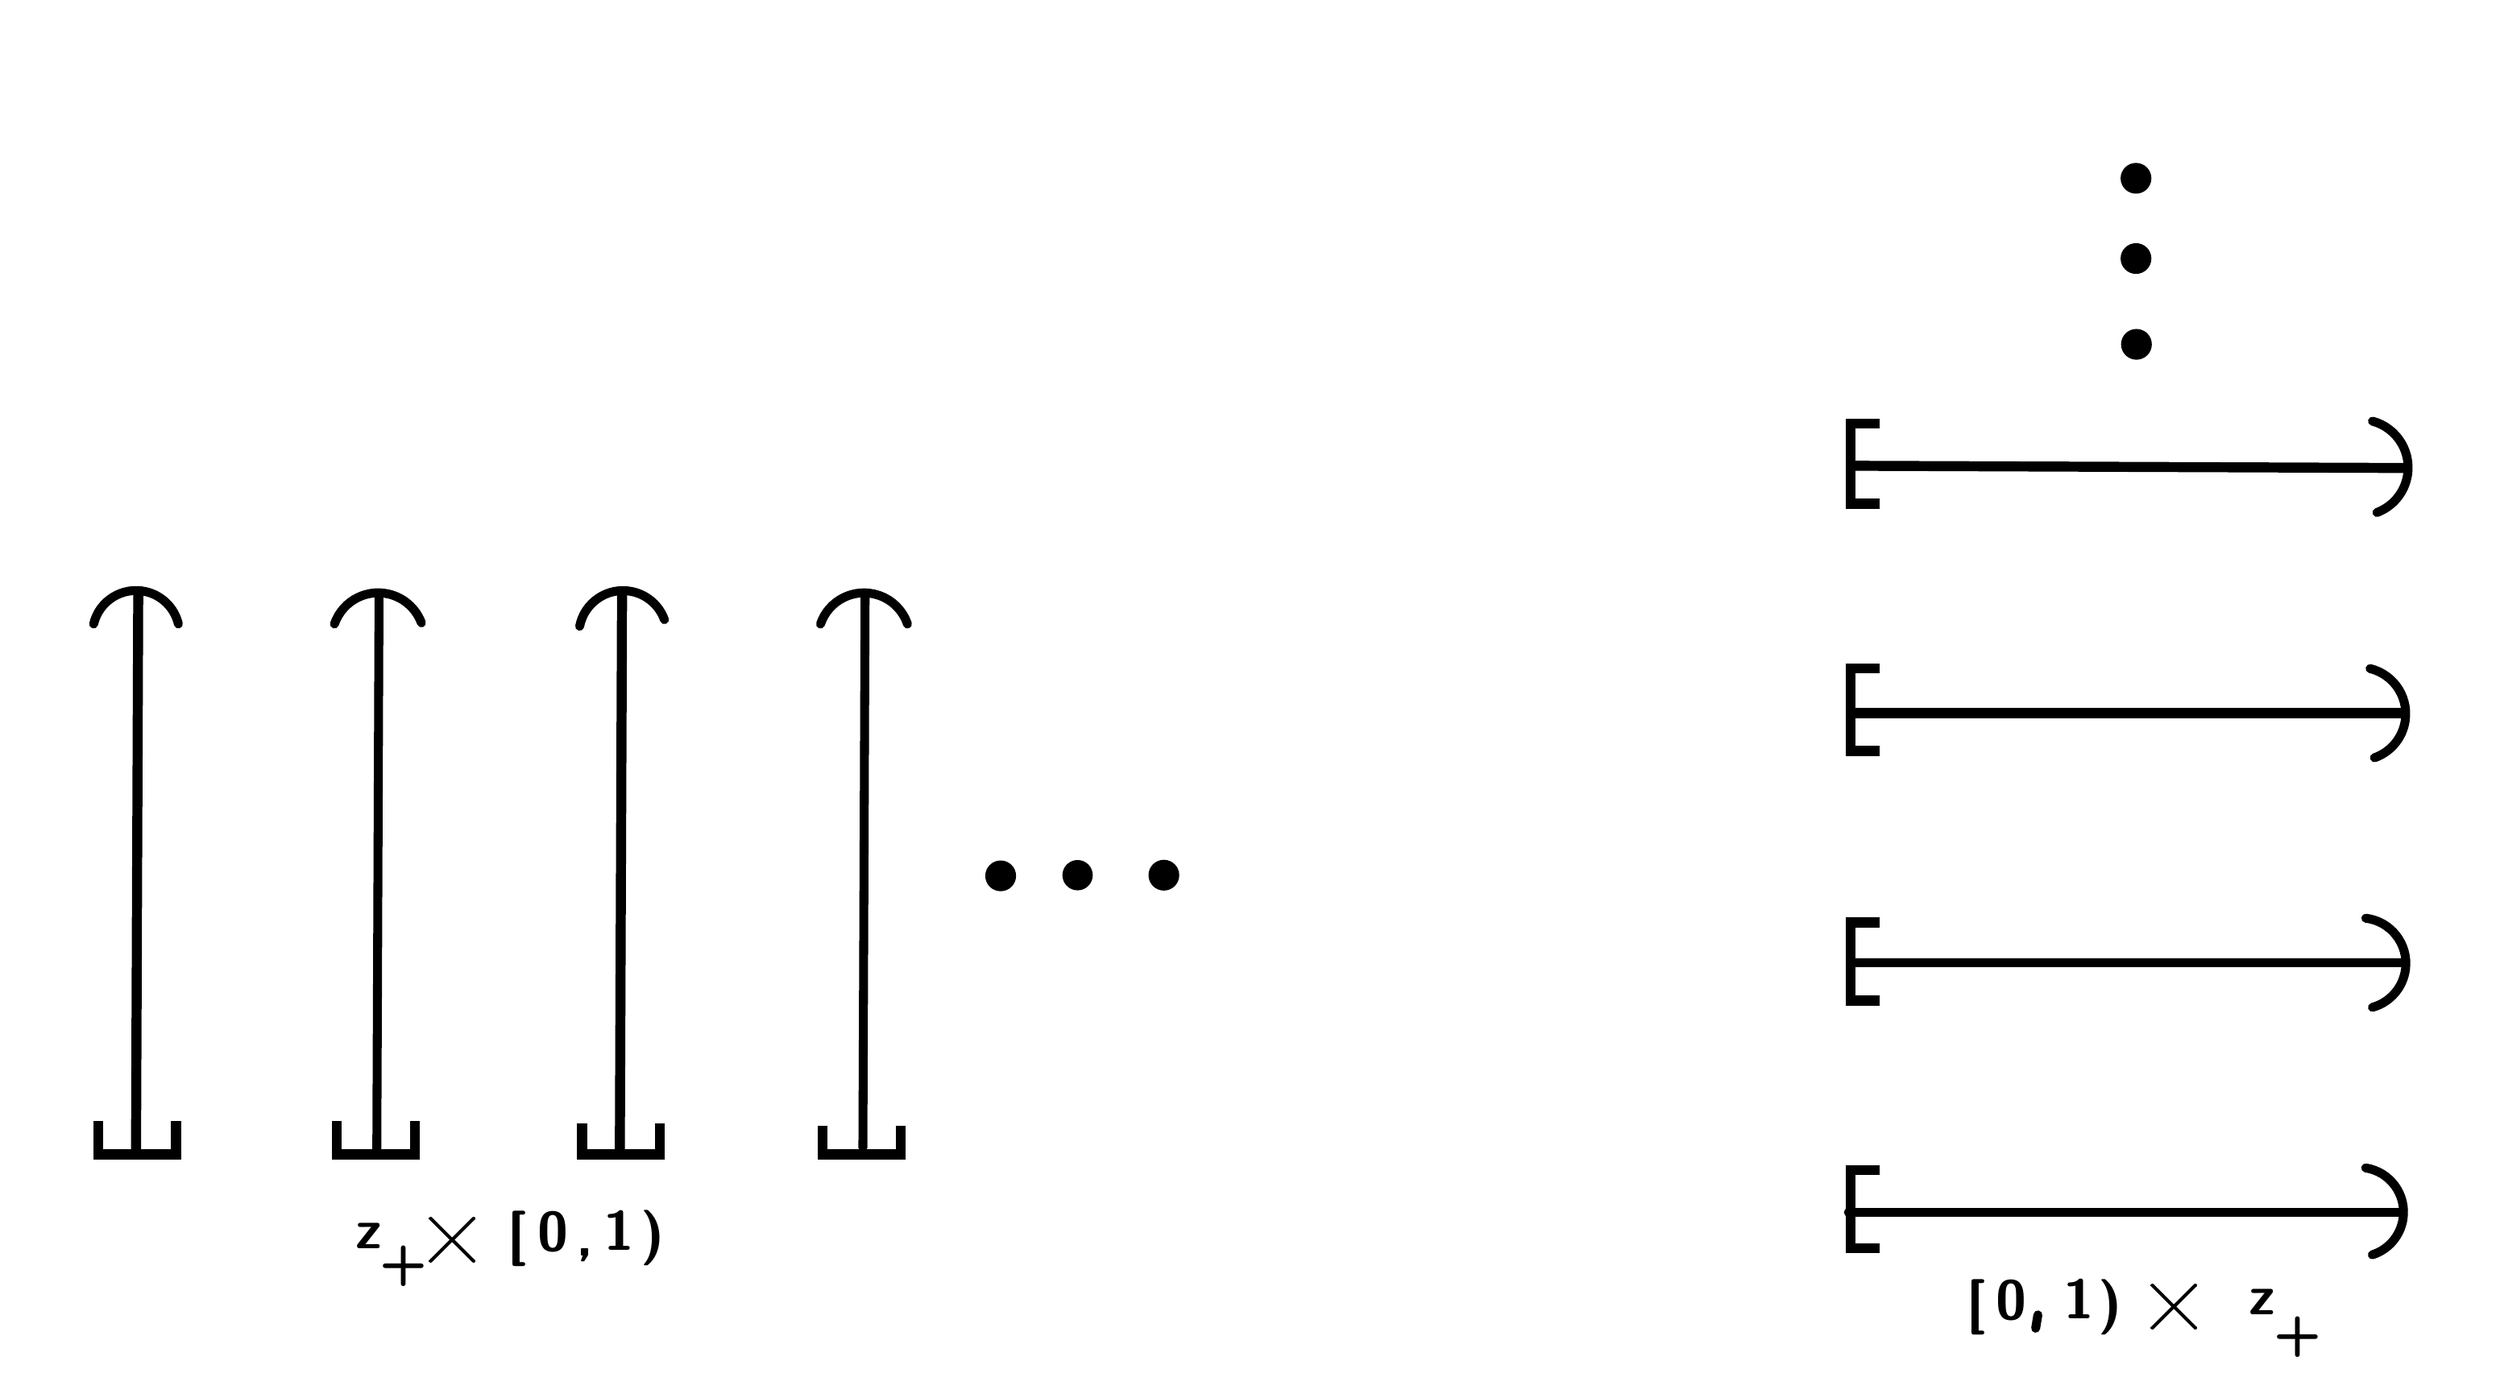
\begin{tikzpicture}[x=1pt, y=-1pt, line width=4.0pt, line cap=round, line join=miter]
  %% 2026-09-25：8 个开区间端原来是**两段手描贝塞尔**，各自改为一条 arc。
  \draw[line width=4pt] (51.0,274.5) ++(-166.7:19.53) arc[start angle=-166.7, end angle=-13.3, radius=19.53];
  \draw[line width=4pt] (159.6,276.7) ++(-161.1:20.70) arc[start angle=-161.1, end angle=-20.3, radius=20.70];
  \draw[line width=4pt] (269.4,274.8) ++(-169.0:19.78) arc[start angle=-169.0, end angle=-20.0, radius=19.78];
  \draw[line width=4pt] (377.5,276.6) ++(-161.4:20.58) arc[start angle=-161.4, end angle=-18.6, radius=20.58];
  \draw[line width=4pt] (1048.1,310.3) ++(-76.5:20.87) arc[start angle=-76.5, end angle=70.8, radius=20.87];
  \draw[line width=4pt] (1048.6,422.3) ++(-83.1:20.44) arc[start angle=-83.1, end angle=74.6, radius=20.44];
  \draw[line width=4pt] (1047.9,533.9) ++(-81.1:20.09) arc[start angle=-81.1, end angle=72.4, radius=20.09];
  \draw[line width=4pt] (1048.5,199.8) ++(-75.1:21.54) arc[start angle=-75.1, end angle=69.5, radius=21.54];
  %% 2026-09-25：**全图 line join 由 round 改为 miter** —— 闭区间端 `[` 必须是**方角**，
  %%   否则与开区间 `)` 分不出来（用户指出）。原来整图 line join=round 把方角磨圆了。
  %%   闭区间端原是 4 段独立笔画（各带**圆线帽**），更把它磨成一团；
  %%   现各写成一条折线 + `line join=miter, line cap=butt`。横杠/臂长由原碎线端点量得。
  \draw[line width=4.5pt, line join=miter, line cap=butt] (176,493) -- (176,508) -- (141,508) -- (141,493);
  \draw[line width=4.5pt, line join=miter, line cap=butt] (34,493) -- (34,508) -- (69,508) -- (69,493);
  \draw[line width=4.5pt, line join=miter, line cap=butt] (251,494) -- (251,508) -- (286,508) -- (286,494);
  \draw[line width=4.5pt, line join=miter, line cap=butt] (359,495) -- (359,508) -- (394,508) -- (394,495);
  %% 2026-09-25：右组 4 个区间号的左端 `[` 帽原来由「斜线 + 竖线 + 贝塞尔」拼成
  %%   （`(832,551)--(819.3,549.3)` 是斜的）⇒ 渲染出台阶。改为一条 `[` 形折线。
  \draw[line width=4.5pt, line join=miter, line cap=butt] (833,290) -- (820,290) -- (820,327) -- (833,327);
  \draw[line width=4.5pt, line join=miter, line cap=butt] (833,180) -- (820,180) -- (820,216) -- (833,216);
  \draw[line width=4.5pt, line join=miter, line cap=butt] (833,404) -- (820,404) -- (820,439) -- (833,439);
  \draw[line width=4.5pt, line join=miter, line cap=butt] (833,515) -- (820,515) -- (820,550) -- (833,550);

  %% ════ 填充区（prims2 的 fills）════

  %% ════ 直线段（prims2 的 strokes）════
  \draw[line width=4.0pt] (160.0,257.0) -- (159.0,507.0);
  \draw[line width=4.5pt] (268.0,507.0) -- (269.0,256.0);
  \draw[line width=4.5pt] (51.0,507.0) -- (52.0,256.0);
  \draw[line width=4.0pt] (904.0,580.0) -- (903.0,586.0);
  \draw[line width=4.5pt] (821.0,310.0) -- (1068.0,310.0);
  \draw[line width=4.0pt] (378.0,257.0) -- (377.0,505.0);
  \draw[line width=4.0pt] (1068.0,422.0) -- (820.0,422.0);
  \draw[line width=4.5pt] (821.0,199.0) -- (1069.0,200.0);
  \draw[line width=4.0pt] (1067.0,534.0) -- (819.0,534.0);

  %% ════ 曲线（prims2 的 curves —— 三段式，坐标同为 (y,x)）════

  %% ════ 实心点 ════
  \fill (948.0,70.0) circle (6.9);
  \fill (948.0,106.0) circle (6.9);
  \fill (948.2,144.5) circle (6.9);
  \fill (438.8,383.0) circle (6.9);
  \fill (473.3,382.7) circle (6.8);
  \fill (512.0,382.7) circle (6.9);

  %% ════ 标签（probe 直接给的 \node 行）════
  %% ⚠ 全部补了 fill=white：文字在最上层，否则与曲线交叉干扰
     \node[anchor=center,inner sep=0pt,fill=white,font=\fontsize{38.0}{47.6}\selectfont] at (155.5,544.5) {\textsf{\textbf{\textit{z}}}};   % box(146,531,17,22)
     \node[anchor=center,inner sep=0pt,fill=white,font=\fontsize{31.3}{39.1}\selectfont] at (222.1,546.0) {\textsf{\textbf{[}}};   % box(216,531,8,28)
     \node[anchor=center,inner sep=0pt,fill=white,font=\fontsize{28.7}{35.9}\selectfont] at (282.9,545.5) {\textsf{\textbf{)}}};   % box(278,531,7,28)
     \node[anchor=center,inner sep=0pt,fill=white,font=\fontsize{30.9}{38.6}\selectfont] at (238.1,542.8) {\textsf{\textbf{0}}};   % box(228,532,15,21)
     \node[anchor=center,inner sep=0pt,fill=white,font=\fontsize{28.2}{35.2}\selectfont] at (267.8,542.5) {\textsf{\textbf{1}}};   % box(260,532,9,20)
     \node[anchor=center,inner sep=0pt,fill=white,font=\fontsize{33.8}{42.3}\selectfont] at (193.1,546.5) {\textsf{\textbf{×}}};   % box(185,536,15,16)
     \node[anchor=center,inner sep=0pt,fill=white,font=\fontsize{34.5}{43.1}\selectfont] at (252.5,553.1) {\textsf{\textbf{,}}};   % box(248,548,5,9)
     \node[anchor=center,inner sep=0pt,fill=white,font=\fontsize{26.0}{32.5}\selectfont] at (171.0,558.0) {\textsf{\textbf{+}}};   % box(163,550,13,13)
     \node[anchor=center,inner sep=0pt,fill=white,font=\fontsize{38.9}{48.6}\selectfont] at (1004.5,574.1) {\textsf{\textbf{\textit{z}}}};   % box(995,560,17,23)
     \node[anchor=center,inner sep=0pt,fill=white,font=\fontsize{29.8}{37.2}\selectfont] at (876.5,576.5) {\textsf{\textbf{[}}};   % box(871,561,7,29)
     \node[anchor=center,inner sep=0pt,fill=white,font=\fontsize{31.6}{39.5}\selectfont] at (892.1,573.3) {\textsf{\textbf{0}}};   % box(882,562,15,22)
     \node[anchor=center,inner sep=0pt,fill=white,font=\fontsize{30.4}{38.0}\selectfont] at (922.5,573.0) {\textsf{\textbf{1}}};   % box(914,562,10,21)
     \node[anchor=center,inner sep=0pt,fill=white,font=\fontsize{30.7}{38.4}\selectfont] at (936.5,576.5) {\textsf{\textbf{)}}};   % box(931,562,8,28)
     \node[anchor=center,inner sep=0pt,fill=white,font=\fontsize{33.8}{42.3}\selectfont] at (965.1,576.5) {\textsf{\textbf{×}}};   % box(957,566,15,16)
     \node[anchor=center,inner sep=0pt,fill=white,font=\fontsize{25.0}{31.2}\selectfont] at (1020.5,590.0) {\textsf{\textbf{+}}};   % box(1013,582,12,13)

  % 钉死画布：否则超出的图元/控制点会把页面撑大，1:1 回比就失准
  \pgfresetboundingbox
  \path[use as bounding box] (0,0) rectangle (1101,607);
\end{tikzpicture}
\end{document}

% ⚠ 待核清单（probe 拿不准，人眼过一遍）：
%   · 未识别/跳过：⑤ 跳过/未识别的字形
